\section{Architettura cache}
La gerarchia di memoria consiste in cache L1 ed L2 collocate in prossimità del core e controllate localmente dal core. La cache L2 può essere privata, o condivisa tra più nodi. L'ultimo livello di cache (LLC) ha un controllore integrato, che funge da interfaccia con gli elementi di ordine superiore. La memoria principale si trova oltre l'LLC. 

\begin{figure}[ht]
    \centering
    \setlength{\fboxrule}{0.5pt} % spessore sottile
    \setlength{\fboxsep}{0pt}    % senza spazio interno
    \fbox{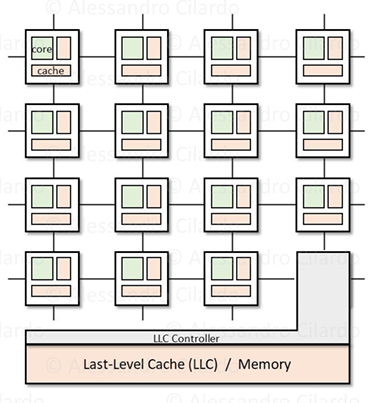
\includegraphics[width=0.5\textwidth]{fig/chapter_3/memory_gerarchia.png}}
\end{figure}

\begin{info}
    Il memory controller che interfaccia LLC e archtiettura di livello superiore (cache più veloci) si può trovare in un nodo separato oppure in uno dei nodi core. LLC è l'ultimo livello in cui ci si deve preoccupare della coerenza, perchè è l'unico compomenente che dialoga con la memoria off-chip.
\end{info}

D'ora in avanti faremo riferimento alla terminologia e alle architettura presentate nella sezione [\ref{sec:richiami_memoria}]. Ogni blocco di memoria in cache è associato ad uno stato, che va opportunamente gestito. Nelle caches e LLC, si estende lo stato associato ad un blocco di qualche bit, e di solito è necessario gestire solo gli stati \textit{stabili} (gli stati \textit{transienti} sono associati a transizioni sospese); Nella memoria principale, notiamo che l'LLC è visto come un insieme di caches locali, e quindi la memoria principale non ha bisogno di stati espliciti: se un blocco non è nell'LLC, il suo stato in memoria è automaticamente \textit{invalido}, ovvero nessuna cache attualmente lo mantiene. 

\noindent Concettualmente, ad ogni blocco è associata una macchina a stati finiti. Lo stato deve essere conservato per tutti i blocchi \textit{cached} lato core, e per tutti i blocchi lato memoria. L'informazione conservata coinvolge solo stati permanenti per quei blocchi che non sono affetti da transazioni. Altrimenti, è necessario conservare informazioni sui \textit{transienti}, che registrano il corrente stato di una transazione. Si usa il MSHR (\textbf{Miss Status Handling Register}) lato core e i TSHRs (\textbf{transaction Status Handling Registers}) lato memoria. 

\begin{figure}[ht]
    \centering
    \setlength{\fboxrule}{0.5pt} % spessore sottile
    \setlength{\fboxsep}{0pt}    % senza spazio interno
    \fbox{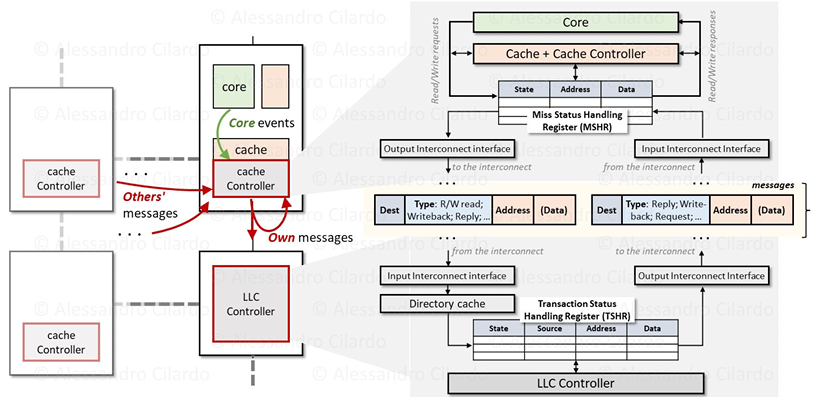
\includegraphics[width=0.75\textwidth]{fig/chapter_3/core_architectures.png}}
\end{figure}

\begin{info}
    Le memorie cache possono anche essere progettate come non coerenti, come nel caso delle \textbf{ScratchPad Memories}: Le scratch pad memories sono memorie veloci di piccole dimensioni integrate all'interno di un processore, pensate per fornire un'area di lavoro temporanea molto più rapida rispetto alla RAM principale. Vengono spesso usate per conservare dati intermedi, variabili critiche o risultati parziali di calcolo che devono essere accessibili con latenze minime. A differenza delle cache, non hanno logiche di gestione automatica della coerenza, ma devono essere programmate esplicitamente: è il programmatore o il compilatore a decidere quali dati caricare e scaricare. Questo implica hardware semplice ma software complesso. Infatti queste memorie hanno uno spazio di indirizzamento autonomo e necessatiano di istruzioni speciali di load/store.
\end{info}

Per applicazioni general purpose è preferibile utilizzare caching trasparente. 


